\chapter{Design}
\section{Interface}
The overall interface works by simply inferring more and more information from the previous step, in a manner like so:

\begin{quote}
	Input (String) $\Rightarrow$ Preprocessor [Separate Lexer, Parser] (String) $\Rightarrow$ Lexer (Token Stream) $\Rightarrow$ Parser (Abstract Syntax Tree) $\Rightarrow$ Semantic Analyzer (Program Attributes, Semantic Syntax Tree) $\Rightarrow$ Code Generation (LLVM IR Module)
\end{quote}

Each step feeds a slimmed-down step to the next parser. The diagram for the workflow can be seen in Figure \ref{fig:diagram}.

\begin{figure}[h!]
	\vspace*{-2cm}
	\makebox[\linewidth]{
		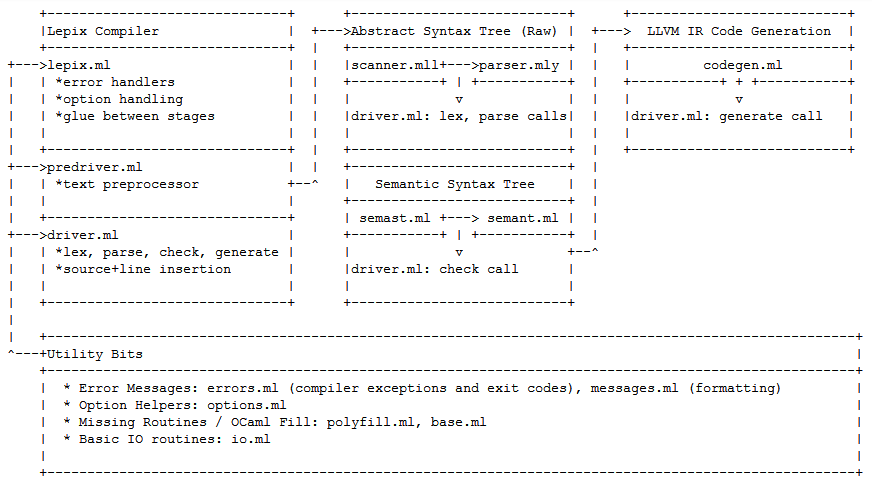
\includegraphics[width=1.3\linewidth]{\detokenize{history/diagram.png}}
	}
	\caption{Compiler and implementation organization.}
	\label{fig:diagram}
\end{figure}

\subsection{Top Level Work-flow}
The way it works is simple at the highest level. Each stage produces one piece of work and hands it off to the next. To support error-reporting, a \lstinline|context| argument is also provided to certain stages, geared to hold tracking information for that stage.

Each component flows from the next, with Preprocessing being an optional step that took in an input file and produced a source string. Because of the way I handled input to the lexer and parser, defining an input channel for either all the text or using an input stream such as stdin was simple.

\subsection{Namespaces}
Namespaces became trivial to implement. Since namespaces themselves are not allowed to be a type -- just a meta-construct for organization -- they needed no physical entry in the final Semantic Syntax Tree. All names of definitions were simply folded to be fully qualified. It would behoove me in further implementation to keep track of the original unqualified name, to ensure that I can easily access both versions of the information easily.

The only other thing that would have come in handy to implement is \lstinline|using namespace| syntax. As of right now, accessing things in namespaces requires fully qualified names. This could get very annoying very quickly, and therefore some form of a \lstinline|using| statement would be good.

\subsection{Bottom-up Type Derivation}
Bottom-up Type Derivation was, essentially, just analyzing the return values of a function. The implementation does not have checkers for expressions that initialize a variable, so the mechanism is not in place for automatic variable deduction, even though the Semantic Syntax Tree will properly tag a variable definition without a type specifier to be of automatically-deduced type.

Thankfully, return values for functions were done. Here, I simply re-ran the semantic analyzer after going through once and getting the return types of all functions and return expressions, and then ran it again to re-gather symbols into the global environment and program attributes. The first Semantic Syntax Tree was thrown out entirely in this process. It is a cheap programmatic way to get the derivations to resolve for all the top-level symbols gathered earlier. A much more effective and composed method would be nice for later, but I had to implement things as fast as possible.

\subsection{Overloading}
Overloading was conceptually difficult to figure out. Many languages have overloading, but a lot of the code examples I had seen were done at runtime. That is, argument arity and strict type matching were done, overloads ranked by that, and then any conversion paths were taken into consideration before determining if a single function call was the best function call. We implemented similar here, without taking into account conversions (because that would require ranking all overloads fully, which is a veritable nightmare to do properly and the source of hundreds -- perhaps thousands -- of bugs in C++, C\#, and other language compilers).

It was important to note that overloading is not part of the original AST, just the Semantic AST as a type for Qualified IDs (only identifiers can be overloaded) and for codegen purposes become mangled names to prevent name lookup confusion (the source of a bug that plagued even past the original deadline and only fixed recently).

\subsection{Error Handling}
True error handling with notices and carat diagnostics were only implemented for the first 3 stages of the compiler: preprocessing, lexing and parsing. Every thing else only has basic exception handlers and no context object to propagate source information or provide carat diagnostics. Thankfully, the test programs were small enough that it was easy to know what was producing errors. The downside is that this means the compiler is not very friendly to users beyond the initial parsing stages, and errors can be even more cryptic than OCaml's.

My primary motivation for good error handling came from OCaml's lacking error messages. Dozens upon dozens of "syntax error" messages that did not even seem to point to the right line, where \lstinline|let| statements would chain well with inner expressions and only error at the end of the program, even though the error that threw off the parser in the first place was much further up in the program. Using \lstinline|and| definitions helped in that regard, but there was still a lot of lost implementation time.

Unfortunately, our error handling again does not do a good job for the semantic errors, which -- once you get used to OCaml's error messages -- are actually quite good. This would take a lot more time to do appropriately, so it is unfortunate that I did not get to do more of it. I really liked implementing carat diagnostics and good error messages with line and character information, and I think it helped me fix the parser and lexer much faster and iterate over it better.

\section{Division of Labor}
I wrote essentially the entire implementation, with little kept from older commits. At one point, Fatima Koly and Akshaan Kakar's for the parser and lexer remained.